\documentclass[11pt]{article}

% ============================================================================
% PACKAGES
% ============================================================================
\usepackage[margin=1in]{geometry}
\usepackage{amsmath,amssymb}
\usepackage{graphicx}
\usepackage{booktabs}
\usepackage{multirow}
\usepackage{hyperref}
\usepackage{xcolor}
\usepackage{listings}
\usepackage{float}
\usepackage{caption}
\usepackage{subcaption}
\usepackage{enumitem}
\usepackage{url}
\usepackage{natbib}
\usepackage{array}
\usepackage{longtable}
\usepackage{tikz}
\usetikzlibrary{shapes.geometric, arrows.meta, positioning, fit, backgrounds}

\hypersetup{
    colorlinks=true,
    linkcolor=blue,
    citecolor=blue,
    urlcolor=blue
}

% Listing style for code/prompts
\lstset{
    basicstyle=\ttfamily\footnotesize,
    breaklines=true,
    frame=single,
    backgroundcolor=\color{gray!10},
    xleftmargin=0.5cm,
    xrightmargin=0.5cm,
    aboveskip=0.5em,
    belowskip=0.5em,
}

% ============================================================================
% TITLE
% ============================================================================

\title{\textbf{TimeToxSV: An LLM-Based Pipeline for Automated Extraction of Time Toxicity from Clinical Trial Protocols}}

\author{
    [Authors -- Placeholder] \\
    [Affiliations -- Placeholder]
}

\date{}

% ============================================================================
% DOCUMENT
% ============================================================================
\begin{document}
\maketitle

% ============================================================================
% ABSTRACT
% ============================================================================
\begin{abstract}
\textbf{Background:} Time toxicity---the cumulative burden of healthcare contact days imposed on patients by clinical trial participation---is an increasingly recognized but understudied dimension of treatment burden. Manually extracting time toxicity from clinical trial protocols is labor-intensive, subjective, and difficult to scale.

\textbf{Methods:} We developed TimeToxSV, an LLM-based pipeline for automated extraction of healthcare contact days from Schedule of Assessments (SoA) tables in clinical trial protocols. Using Google's Gemini models, the pipeline operates in three stages: (1) summary extraction, where Gemini 2.5 Flash identifies and extracts SoA-relevant pages from full-length protocol PDFs; (2) time toxicity extraction, where Gemini 3.0 Flash quantifies healthcare contact days at six cumulative timepoints (screening, 1, 3, 6, 9, and 12 months) for each treatment arm; and (3) multi-run consensus, where position-based arm matching and median aggregation across three independent extraction runs produces stable estimates. We validated the extraction pipeline against 20 programmatically generated synthetic schedules (40 arms, 240 comparisons) with clinician-verified ground truth. We evaluated two extraction architectures---a single-pass vanilla approach and a two-stage structure-then-count approach---and assessed reproducibility through 5-run stability testing on 100 real-world protocols and 3-run stability testing on all 644 real-world protocols.

\textbf{Results:} On synthetic data, the two-stage pipeline achieved 100\% clinical accuracy ($\pm$3 days) with a mean absolute error of 0.81 days, compared to 41.5\% clinical accuracy and 9.0-day MAE for the vanilla pipeline. However, on real-world protocols, the vanilla pipeline demonstrated markedly superior reproducibility: 93.7\% clinical stability (IQR $\leq$ 3 days) across 5 runs on 100 protocols and 95.3\% across 3 runs on all 644 protocols, with 82.0\% achieving perfect stability (IQR = 0). The two-stage pipeline exhibited high inter-run variance on real protocols despite its synthetic accuracy. The production pipeline (vanilla + 3-run consensus) was applied to 644 real-world oncology trial protocols, successfully extracting time toxicity for 1,288 treatment arms across multiple disease sites and treatment modalities.

\textbf{Conclusions:} TimeToxSV enables scalable, reproducible quantification of time toxicity from clinical trial protocols. The pipeline demonstrates that extraction stability on real-world data, rather than accuracy on synthetic benchmarks, is the decisive factor for production deployment. Code is available at [GitHub URL].
\end{abstract}

\textbf{Keywords:} time toxicity, large language models, clinical trial protocols, healthcare contact days, schedule of assessments, automated extraction

% ============================================================================
% 1. INTRODUCTION
% ============================================================================
\section{Introduction}

Clinical trial participation imposes substantial time demands on patients beyond the direct effects of treatment itself. These demands---including clinic visits, laboratory tests, imaging studies, and other protocol-mandated activities---constitute what has been termed ``time toxicity,'' defined as the cumulative number of days requiring in-person healthcare contact~\citep{gupta2022time}. Unlike traditional toxicity endpoints that focus on physical side effects, time toxicity captures the temporal burden that can affect quality of life, employment, caregiving responsibilities, and ultimately trial participation decisions.

Despite growing recognition of time toxicity as a meaningful patient-centered outcome, its systematic quantification remains challenging. The Schedule of Assessments (SoA) table---a dense, multi-page document embedded within clinical trial protocols---specifies all required activities, their timing, and their applicability to each treatment arm. Manually extracting healthcare contact days from these tables requires: (1) mapping cycle-based schedules to calendar days, (2) expanding grouped column headers (e.g., ``Cycles 4--12'') into individual cycles, (3) distinguishing arm-specific assessments from universal ones, and (4) accumulating unique contact days across cumulative time windows while avoiding double-counting. This process is time-consuming, error-prone, and difficult to standardize across reviewers.

Recent advances in large language models (LLMs) have demonstrated remarkable capabilities in processing complex structured documents, including medical texts and tabular data. LLMs can parse visual table layouts, understand domain-specific terminology, and perform multi-step reasoning over structured content---skills directly applicable to SoA table interpretation. However, deploying LLMs for clinical data extraction introduces challenges of its own: output variability across runs, sensitivity to prompt design, and the difficulty of validating extractions at scale when ground truth is scarce.

In this work, we present TimeToxSV, an end-to-end LLM-based pipeline for automated extraction of time toxicity from clinical trial protocols. Our contributions include:

\begin{enumerate}[leftmargin=*]
    \item A complete pipeline from raw protocol PDFs to structured time toxicity data, using Gemini models for both document preprocessing and data extraction.
    \item A programmatically generated ground truth dataset of 20 synthetic SoA schedules with clinician-verified time toxicity values, enabling systematic validation.
    \item A comparative evaluation of two extraction architectures---single-pass (vanilla) and two-stage (structure-then-count)---revealing a critical trade-off between synthetic accuracy and real-world stability.
    \item A position-based consensus mechanism that handles LLM-generated arm name instability across runs, enabling robust multi-run aggregation.
    \item Application of the production pipeline to 644 real-world oncology trial protocols, demonstrating feasibility at scale.
\end{enumerate}

% ============================================================================
% 2. DATA COLLECTION AND PREPROCESSING
% ============================================================================
\section{Data Collection and Preprocessing}

\subsection{Protocol Acquisition}

We compiled a dataset of 649 clinical trial protocol documents from ClinicalTrials.gov, spanning multiple oncology disease sites including breast, thoracic, gastrointestinal, genitourinary, gynecologic, head and neck, skin, central nervous system, and hematologic malignancies. Protocols were selected based on the availability of full-text documents with Schedule of Assessments tables.

\subsection{Summary Extraction}

Full-length clinical trial protocols typically span 100--400 pages, of which only 5--15 pages contain the SoA table and related scheduling information. To reduce input size and improve extraction accuracy, we developed an automated summary extraction stage using Google's Gemini 2.5 Flash model.

For each protocol PDF, the summary extraction pipeline:
\begin{enumerate}[leftmargin=*]
    \item Uploads the full PDF to the Gemini API.
    \item Prompts the model to identify pages containing SoA tables, visit schedules, assessment timing, or related scheduling information. The prompt instructs the model to be liberal in page identification to avoid missing relevant content.
    \item Generates a consolidated summary PDF containing: (a) a concise trial summary (study design, treatment arms, duration), and (b) the identified SoA pages plus one surrounding page on each side for context.
\end{enumerate}

The summary extraction uses forced JSON output via \texttt{response\_mime\_type="application/json"} with a structured schema, temperature 0.0, and top-$p$ 0.95. Processing time averages 2--3 minutes per protocol. Of the 649 protocols processed, summaries were successfully generated for 646, yielding a 99.5\% success rate.

Table~\ref{tab:dataset_overview} summarizes the dataset characteristics.

\begin{table}[H]
\centering
\caption{Dataset Overview}
\label{tab:dataset_overview}
\begin{tabular}{lr}
\toprule
\textbf{Characteristic} & \textbf{Value} \\
\midrule
Total protocols collected & 649 \\
Protocols with successful summary extraction & 644 \\
Summary extraction success rate & 99.5\% \\
Summary extraction model & Gemini 2.5 Flash \\
Average processing time per protocol & 2--3 min \\
Average SoA pages identified per protocol & 5--15 \\
Disease sites represented & 11 \\
\bottomrule
\end{tabular}
\end{table}

% ============================================================================
% 3. GROUND TRUTH DEVELOPMENT
% ============================================================================
\section{Ground Truth Development}

\subsection{Synthetic Schedule Generation}

To enable systematic validation of extraction pipelines, we developed a programmatic generator for synthetic SoA schedules. The generator (\texttt{generate\_schedules.py}, 1,284 lines) creates realistic HTML-rendered schedules with known ground truth values, enabling precise accuracy measurement without the ambiguity inherent in real-world protocol interpretation.

Each synthetic schedule includes:
\begin{itemize}[leftmargin=*]
    \item A complete SoA table with realistic assessment categories (administrative, clinical, laboratory, cardiac, safety, treatment, imaging, and patient-reported outcomes).
    \item Two treatment arms (intervention and control) with distinct visit schedules.
    \item Cycle-based timing with configurable cycle lengths (7, 21, 28, or 35 days).
    \item Treatment durations ranging from 2 to 12 months.
    \item A legend section specifying arm-specific visit patterns.
    \item Footnotes, headers, and formatting consistent with real clinical trial protocols.
    \item Disease-specific assessments appropriate to each tumor type.
\end{itemize}

We generated 20 synthetic schedules spanning 8 oncology disease categories (breast, thoracic, gastrointestinal, genitourinary, head \& neck, melanoma, gynecologic, and sarcoma) with three complexity levels: simple ($n=5$, single visit day per cycle), moderate ($n=10$, two visit days per cycle), and complex ($n=5$, three visit days per cycle). Five distinct visual styles were used to test robustness to formatting variation. Schedules incorporated diverse treatment modalities including systemic therapy, radiation, and surgery.

\subsection{Ground Truth Calculation}

Ground truth healthcare contact days were computed deterministically from each schedule's configuration parameters:
\begin{enumerate}[leftmargin=*]
    \item Treatment visit days were mapped from cycle-based schedules to absolute calendar days.
    \item Imaging days were added at protocol-specified intervals.
    \item End-of-treatment (EOT) and follow-up visits at 9 and 12 months were included.
    \item Unique calendar days were counted at each cumulative timepoint (screening, 1, 3, 6, 9, 12 months).
\end{enumerate}

This yielded 40 arms $\times$ 6 timepoints = 240 ground truth comparisons. Table~\ref{tab:synthetic_characteristics} summarizes the synthetic dataset.

\begin{table}[H]
\centering
\caption{Synthetic Schedule Characteristics}
\label{tab:synthetic_characteristics}
\begin{tabular}{lr}
\toprule
\textbf{Characteristic} & \textbf{Value} \\
\midrule
Total schedules & 20 \\
Total arms & 40 (20 intervention, 20 control) \\
Total ground truth comparisons & 240 \\
Disease categories & 8 \\
Complexity: Simple / Moderate / Complex & 5 / 10 / 5 \\
Cycle lengths & 7, 21, 28, 35 days \\
Treatment durations & 2--12 months \\
Visual style variants & 5 \\
Treatment modalities & Systemic, Radiation, Surgery \\
\bottomrule
\end{tabular}
\end{table}

\subsection{Ground Truth Verification}

The programmatically generated ground truth values were independently verified by multiple reviewers, including a clinician expert who assessed the clinical plausibility of the synthetic schedules and confirmed the correctness of the calculated contact days. This verification ensured that both the schedule designs and the ground truth calculations accurately reflected real-world clinical trial visit patterns.

% ============================================================================
% 4. LLM PIPELINE DESIGN
% ============================================================================
\section{LLM Pipeline Design}

We evaluated two extraction architectures, both using Google's Gemini 3.0 Flash (\texttt{gemini-3-flash-preview}) as the base model with temperature 0.1 to balance accuracy and determinism.

\subsection{Vanilla Pipeline (Primary)}

The vanilla pipeline performs single-pass extraction, providing the model with a summary SoA PDF and a structured prompt that requests direct quantification of healthcare contact days. The prompt (76 lines of instruction, excluding the JSON output template) specifies:

\begin{enumerate}[leftmargin=*]
    \item \textbf{Definitions:} Healthcare contact day definition, six cumulative time windows (screening through 12 months), and the instruction to count each unique calendar day once regardless of the number of assessments.
    \item \textbf{Extraction rules:} Five key rules covering arm identification, cycle-to-calendar mapping, grouped column expansion, unique day counting, and arm-specific visit handling (e.g., superscript markers like $X^A$).
    \item \textbf{Category definitions:} Four categories of healthcare contact---core treatment, imaging/diagnostics, labs, and clinic visits---with the note that a single day may span multiple categories.
    \item \textbf{Output format:} Strict JSON schema specifying arm name, intervention type, healthcare contact days at each timepoint, category breakdown, and extraction notes (cycle length, treatment duration, visit pattern, disease).
\end{enumerate}

The model receives the PDF as a visual input and produces a JSON response. Three retry attempts with exponential backoff handle transient API failures. Listing~\ref{lst:vanilla_prompt_excerpt} shows a condensed excerpt of the prompt.

\begin{lstlisting}[caption={Condensed excerpt of the vanilla extraction prompt.}, label={lst:vanilla_prompt_excerpt}]
You are an expert clinical trial protocol analyst.
Your task is to extract healthcare contact days
from the Schedule of Assessments (SoA) table.

## DEFINITIONS
**Healthcare Contact Day**: Any calendar day requiring
in-person contact with the healthcare system.
Count each unique calendar day ONCE.

**Time Windows** (cumulative):
- screening: All pre-treatment visits
- 1_month: Day 1 through Day 30
- 3_months: Day 1 through Day 90
...
- 12_months: Day 1 through Day 365

## EXTRACTION RULES
1. Identify all treatment arms
2. Map cycle structure to calendar days
3. CRITICAL: Expand grouped columns (e.g., "C4-C12")
4. Count unique visit days
5. Handle arm-specific visits (superscripts)

## OUTPUT FORMAT
Return ONLY valid JSON: [{"arm_name": "...",
  "healthcare_contact_days": {...}, ...}]
\end{lstlisting}

\subsection{Two-Stage Pipeline (Alternative)}

The two-stage pipeline decomposes extraction into two sequential LLM calls:

\textbf{Stage 1 --- Structure Extraction:} The model extracts the structural parameters of the SoA table, including: cycle length in days, visit days per cycle for each arm, treatment duration, special visit information (screening days, EOT visit, follow-up visits), and disease type. The output is a structured JSON object capturing the schedule's ``blueprint'' without performing any counting. This stage uses forced JSON output (\texttt{response\_mime\_type="application/json"}).

\textbf{Stage 2 --- Count Calculation:} The extracted structure from Stage 1, formatted as JSON, is provided alongside the original PDF as context for a second LLM call. This call performs the arithmetic: mapping cycles to calendar days, applying visit patterns, and accumulating unique contact days at each timepoint. The prompt includes explicit calculation rules (e.g., ``Total cycles = floor(treatment\_duration\_months $\times$ 30 / cycle\_length\_days)'').

The rationale for decomposition was to separate the perceptual task (reading the table) from the computational task (counting days), hypothesizing that this division would reduce errors. As described in Section~\ref{sec:stability}, while this approach achieved superior accuracy on synthetic data, it exhibited unacceptable variability on real-world protocols.

% ============================================================================
% 5. VALIDATION ON SYNTHETIC DATA
% ============================================================================
\section{Validation on Synthetic Data}

\subsection{Evaluation Metrics}

We evaluated both pipelines using three metrics computed across all 240 ground truth comparisons (20 schedules $\times$ 2 arms $\times$ 6 timepoints):

\begin{itemize}[leftmargin=*]
    \item \textbf{Exact Match Accuracy:} Percentage of extractions matching the ground truth exactly.
    \item \textbf{Clinical Accuracy ($\pm$3 days):} Percentage of extractions within 3 days of the ground truth, reflecting the threshold at which differences are clinically meaningful.
    \item \textbf{Mean Absolute Error (MAE):} Average absolute difference between extracted and ground truth values, in days.
\end{itemize}

\subsection{Results}

Table~\ref{tab:synthetic_validation} presents the validation results. The two-stage pipeline substantially outperformed the vanilla pipeline on all synthetic accuracy metrics, achieving perfect clinical accuracy. However, as Section~\ref{sec:stability} demonstrates, these synthetic metrics did not predict real-world performance.

\begin{table}[H]
\centering
\caption{Validation Results on 20 Synthetic Schedules (240 Comparisons)}
\label{tab:synthetic_validation}
\begin{tabular}{lccc}
\toprule
\textbf{Pipeline} & \textbf{Exact Match} & \textbf{Clinical Accuracy ($\pm$3d)} & \textbf{MAE (days)} \\
\midrule
Vanilla (single-pass) & 0.3\% & 41.5\% & 9.0 \\
Two-Stage (structure $\to$ count) & 29.2\% & 100.0\% & 0.81 \\
\bottomrule
\end{tabular}
\end{table}

The vanilla pipeline's low synthetic accuracy is attributable to the inherent difficulty of performing multi-step arithmetic (cycle mapping, grouped column expansion, cumulative counting) in a single LLM call. The model frequently miscounts visits in grouped columns or makes errors in cycle-to-day conversion. In contrast, the two-stage pipeline benefits from explicit structural extraction followed by guided calculation, reducing the cognitive load on each individual call.

% ============================================================================
% 6. STABILITY AND REPRODUCIBILITY TESTING
% ============================================================================
\section{Stability and Reproducibility Testing}
\label{sec:stability}

\subsection{Motivation}

While synthetic accuracy measures correctness against known ground truth, production deployment requires a different property: \emph{reproducibility}. If the same protocol yields substantially different time toxicity values across independent extraction runs, the resulting dataset cannot support reliable downstream analysis. We therefore conducted systematic stability testing on real-world protocols.

\subsection{Phase 1: Pilot Stability Study (5 Runs, 100 Protocols)}

We first compared both pipelines on a pilot set of real-world protocols. Using 5 CTGProtocol summary PDFs, we ran each pipeline 5 times and measured the inter-quartile range (IQR) of the 12-month healthcare contact day count across runs for each arm.

The two-stage pipeline exhibited substantial inter-run variability on real protocols. For example, one protocol arm produced values of [94, 473, 473, 540, 543] across 5 two-stage runs (IQR = 258.0), while the same arm under the vanilla pipeline produced [99, 105, 106, 106, 106] (IQR = 4.0). Another protocol yielded two-stage values of [27, 53, 53, 53, 53] (IQR = 13.0) versus vanilla values of [8, 8, 8, 8, 8] (IQR = 0.0).

This discrepancy---high synthetic accuracy but high real-world variability for the two-stage pipeline---reflects a fundamental challenge: real-world SoA tables are far more heterogeneous than synthetic schedules. Ambiguous column headers, inconsistent formatting, multi-page tables, and complex footnotes create interpretation variability that is amplified by the two-stage pipeline's reliance on accurate structural extraction in Stage~1.

We then extended stability testing to 100 real-world protocols with 5 independent vanilla runs. Table~\ref{tab:stability_phase1} presents the results.

\begin{table}[H]
\centering
\caption{Vanilla Pipeline Stability: 5 Runs on 100 Real-World Protocols}
\label{tab:stability_phase1}
\begin{tabular}{lrr}
\toprule
\textbf{Stability Category} & \textbf{Arms} & \textbf{Percentage} \\
\midrule
Perfect Stability (IQR = 0) & 417 & 77.2\% \\
Clinical Stability (IQR $\leq$ 3) & 506 & 93.7\% \\
High Variance (IQR $>$ 3) & 34 & 6.3\% \\
\midrule
\textbf{Total arms analyzed} & \textbf{540} & \\
\bottomrule
\end{tabular}
\end{table}

\subsection{Phase 2: Full-Scale Stability (3 Runs, 644 Protocols)}

Based on the pilot results, we selected the vanilla pipeline for production deployment and ran 3 independent extractions on all 644 successfully preprocessed protocols. Table~\ref{tab:stability_phase2} presents the full-scale stability results.

\begin{table}[H]
\centering
\caption{Vanilla Pipeline Stability: 3 Runs on 644 Real-World Protocols}
\label{tab:stability_phase2}
\begin{tabular}{lrr}
\toprule
\textbf{Stability Category} & \textbf{Arms} & \textbf{Percentage} \\
\midrule
Perfect Stability (IQR = 0) & 2,172 & 82.0\% \\
Clinical Stability (IQR $\leq$ 3) & 2,524 & 95.3\% \\
High Variance (IQR $>$ 3) & 125 & 4.7\% \\
\midrule
\textbf{Total arms analyzed} & \textbf{2,649} & \\
\bottomrule
\end{tabular}
\end{table}

The improvement from 93.7\% to 95.3\% clinical stability when moving from 5 runs on 100 protocols to 3 runs on 644 protocols likely reflects both the natural variance reduction with fewer runs and the broader protocol sample smoothing out edge cases.

\subsection{Stability Metrics}

We define clinical stability as follows:
\begin{itemize}[leftmargin=*]
    \item \textbf{Perfect Stability (IQR = 0):} All runs produced identical 12-month contact day counts for this arm.
    \item \textbf{Clinical Stability (IQR $\leq$ 3):} The interquartile range of 12-month counts is at most 3 days---a threshold below which differences are not clinically meaningful.
    \item \textbf{High Variance (IQR $>$ 3):} Substantial disagreement across runs, flagging arms for potential review.
\end{itemize}

% ============================================================================
% 7. PRODUCTION PIPELINE AND CONSENSUS
% ============================================================================
\section{Production Pipeline and Consensus}

\subsection{Pipeline Architecture}

Based on the validation and stability results, we adopted the vanilla pipeline with 3-run consensus as the production configuration. Figure~\ref{fig:pipeline_overview} illustrates the complete pipeline architecture.

\begin{figure}[H]
\centering
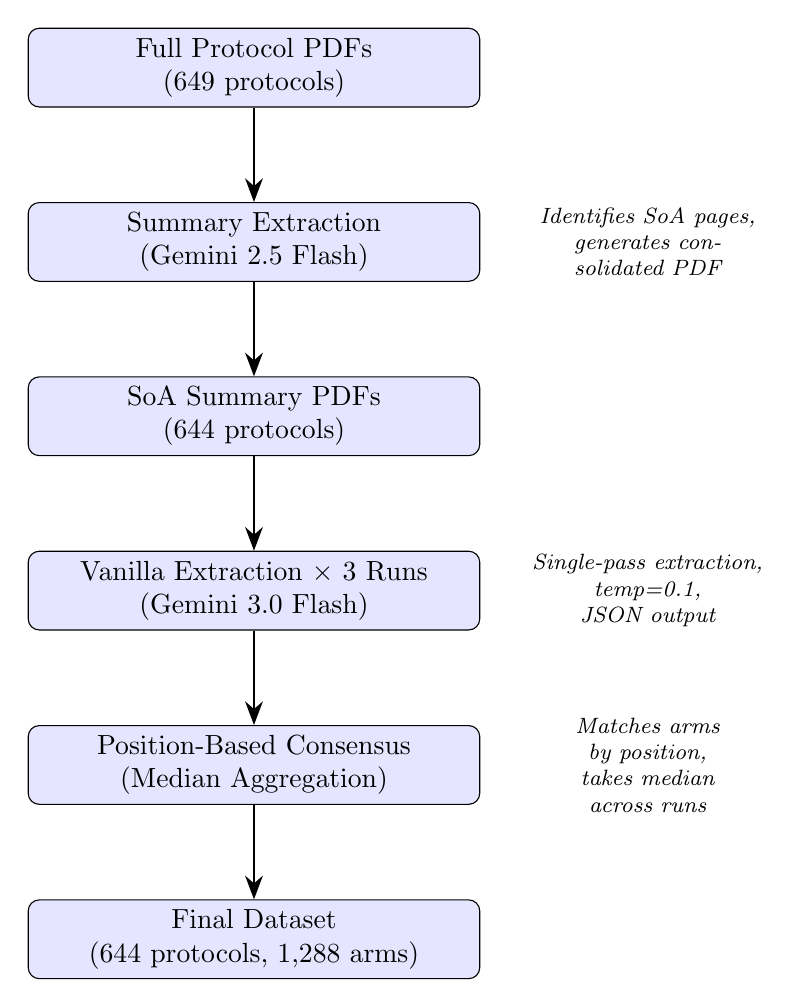
\begin{tikzpicture}[
    node distance=1.2cm,
    block/.style={rectangle, draw, fill=blue!10, text width=5.5cm, text centered, rounded corners, minimum height=1cm},
    arrow/.style={-{Stealth[length=3mm]}, thick},
    label/.style={font=\footnotesize\itshape, text width=3cm, text centered}
]
    % Nodes
    \node[block] (pdf) {Full Protocol PDFs\\(649 protocols)};
    \node[block, below=of pdf] (summary) {Summary Extraction\\(Gemini 2.5 Flash)};
    \node[block, below=of summary] (soa) {SoA Summary PDFs\\(644 protocols)};
    \node[block, below=of soa] (run1) {Vanilla Extraction $\times$ 3 Runs\\(Gemini 3.0 Flash)};
    \node[block, below=of run1] (consensus) {Position-Based Consensus\\(Median Aggregation)};
    \node[block, below=of consensus] (output) {Final Dataset\\(644 protocols, 1,288 arms)};

    % Arrows
    \draw[arrow] (pdf) -- (summary);
    \draw[arrow] (summary) -- (soa);
    \draw[arrow] (soa) -- (run1);
    \draw[arrow] (run1) -- (consensus);
    \draw[arrow] (consensus) -- (output);

    % Labels
    \node[label, right=0.5cm of summary] {Identifies SoA pages,\\generates consolidated PDF};
    \node[label, right=0.5cm of run1] {Single-pass extraction,\\temp=0.1, JSON output};
    \node[label, right=0.5cm of consensus] {Matches arms by position,\\takes median across runs};
\end{tikzpicture}
\caption{TimeToxSV production pipeline architecture.}
\label{fig:pipeline_overview}
\end{figure}

\subsection{Position-Based Consensus Mechanism}

A key challenge in multi-run LLM extraction is arm name instability: the same treatment arm may be labeled differently across runs (e.g., ``Arm A (Pembrolizumab + Chemotherapy)'' vs.\ ``Pembrolizumab + Chemotherapy Arm'' vs.\ ``Treatment Arm A: Pembro/Chemo''). Standard name-based matching fails in this scenario.

We address this through position-based matching:
\begin{enumerate}[leftmargin=*]
    \item Within each run, arms are grouped by \texttt{(filename, intervention\_type)}.
    \item Within each group, arms are sorted by their 12-month healthcare contact day count.
    \item A positional index (\texttt{pos\_idx}) is assigned based on this sorted order.
    \item Consensus is computed by grouping across runs by \texttt{(filename, intervention\_type, pos\_idx)} and taking the median of each timepoint.
\end{enumerate}

This approach leverages the insight that even when arm names vary, the relative ordering of arms by time toxicity burden is stable. The intervention type (intervention vs.\ control) is normalized during preprocessing (e.g., ``placebo'' $\to$ ``control'', ``active\_comparator'' $\to$ ``intervention'').

Table~\ref{tab:consensus_stats} summarizes the consensus dataset.

\begin{table}[H]
\centering
\caption{Production Consensus Dataset Statistics}
\label{tab:consensus_stats}
\begin{tabular}{lr}
\toprule
\textbf{Metric} & \textbf{Value} \\
\midrule
Protocols processed & 644 \\
Total consensus arms & 1,288 \\
Arms with 3 concordant runs & majority \\
Extraction model & Gemini 3.0 Flash \\
Extraction temperature & 0.1 \\
Extraction runs per protocol & 3 \\
Consensus method & Median aggregation \\
Average processing time per extraction & $\sim$4 min \\
\bottomrule
\end{tabular}
\end{table}

\subsection{Cost and Runtime}

The full production pipeline cost is dominated by API calls to the Gemini models. Summary extraction (Gemini 2.5 Flash) processes each protocol in approximately 2--3 minutes. Each vanilla extraction run (Gemini 3.0 Flash) takes approximately 4 minutes per protocol. With 3 runs across 644 protocols, the total extraction time is approximately 128 hours of sequential processing (reducible through parallelization). The Gemini API pricing makes the total cost well under \$100 for the complete dataset, making the approach economically viable for large-scale studies.

% ============================================================================
% 8. APPLICATION
% ============================================================================
\section{Application}

To demonstrate the pipeline's utility, we applied the production consensus dataset to a landscape analysis of time toxicity across oncology clinical trials. The full clinical analysis---including descriptive statistics, comparative analyses across disease sites and treatment modalities, temporal trends, multivariable regression, and component analysis---is presented in a companion paper.

Briefly, the pipeline enabled analysis of time toxicity patterns across 644 protocols spanning 11 disease sites, multiple treatment modalities (chemotherapy, immunotherapy, targeted therapy, endocrine therapy, radiation, and procedures), and trial start years from 1994 to 2021. The median 12-month time toxicity across all intervention arms was quantified, and systematic differences by disease site, treatment type, and funding source were characterized---analyses that would be infeasible through manual extraction at this scale.

% ============================================================================
% 9. DISCUSSION
% ============================================================================
\section{Discussion}

\subsection{Accuracy vs.\ Stability Trade-off}

The central finding of this work is the critical distinction between synthetic accuracy and real-world stability. The two-stage pipeline achieved perfect clinical accuracy on synthetic schedules but exhibited unacceptable variability on real-world protocols. Conversely, the vanilla pipeline showed modest synthetic accuracy but remarkable stability---95.3\% of arms had an IQR $\leq$ 3 days across independent runs.

This divergence has a straightforward explanation. Synthetic schedules have unambiguous structure: clear column headers, explicit legends, and well-defined visit patterns. The two-stage pipeline excels when the structural extraction step can cleanly parse this structure. Real-world protocols, however, contain multi-page tables with complex footnotes, ambiguous column groupings, inconsistent notation, and formatting artifacts. In this environment, small variations in structural extraction at Stage~1 cascade into large counting differences at Stage~2. The vanilla pipeline, by avoiding explicit structural decomposition, is more robust to these sources of ambiguity---it treats extraction as a holistic task, reducing the number of failure points.

\subsection{Design Decisions}

Several design decisions shaped the pipeline:

\textbf{Temperature selection:} We used temperature 0.1 throughout extraction. Lower temperatures (0.0) with forced JSON output were tested during development but did not consistently improve stability, while they occasionally caused the model to produce malformed outputs. Temperature 0.1 provided a balance between determinism and output quality.

\textbf{Prompt design:} The vanilla prompt underwent iterative refinement. Key additions included the explicit instruction to expand grouped columns (``CRITICAL -- Expand grouped columns''), the specification that time windows are cumulative, and the category breakdown requirement. Each addition addressed a systematic error pattern observed during development.

\textbf{Three-run consensus:} Three runs were chosen as a pragmatic balance between stability and cost. Increasing from 3 to 5 runs would provide marginal stability improvement (as evidenced by the 93.7\% vs.\ 95.3\% comparison) at a 67\% increase in cost.

\subsection{Limitations}

Several limitations should be acknowledged:

\begin{enumerate}[leftmargin=*]
    \item \textbf{Single LLM family:} All extraction uses Google's Gemini models. While Gemini 3.0 Flash demonstrated good performance, comparative evaluation against other LLM families (GPT-4, Claude) was not conducted with formal benchmarking.
    \item \textbf{Synthetic-only formal validation:} Clinical accuracy was formally validated only against synthetic schedules. Real-world validation relied on stability testing and informal spot-checking against manually reviewed protocols rather than a comprehensive gold standard.
    \item \textbf{Systematic bias:} The vanilla pipeline may systematically under- or over-count healthcare contact days. While the consensus mechanism reduces random error, it cannot correct consistent directional bias across runs.
    \item \textbf{Protocol heterogeneity:} Extremely complex protocols (e.g., multi-phase adaptive designs with dose-escalation cohorts) may exceed the pipeline's extraction capability, contributing to the 4.7\% of arms with high variance.
    \item \textbf{Temporal coverage:} The pipeline extracts contact days up to 12 months. Longer-term follow-up visits beyond 12 months are not captured.
\end{enumerate}

\subsection{Comparison to Related Work}

LLM-based information extraction from medical documents is an active area of research. Prior work has demonstrated the feasibility of using LLMs for tasks such as extracting structured data from clinical notes, annotating medical literature, and processing clinical trial registries. Our work extends this line of research to a specific, previously unautomated task---time toxicity quantification from SoA tables---that requires both visual table parsing and multi-step arithmetic reasoning.

The stability-focused evaluation framework we employ is less common in the LLM extraction literature, which typically emphasizes accuracy against gold standards. Our finding that stability on heterogeneous real-world data is a better predictor of production utility than accuracy on controlled benchmarks may generalize to other LLM-based extraction tasks.

% ============================================================================
% 10. CONCLUSION
% ============================================================================
\section{Conclusion}

We presented TimeToxSV, an LLM-based pipeline for automated extraction of time toxicity from clinical trial protocol SoA tables. The pipeline combines Gemini-based summary extraction, vanilla single-pass time toxicity extraction, and position-based multi-run consensus to produce stable, scalable quantification of healthcare contact days.

Our evaluation revealed a critical insight for LLM deployment in clinical data extraction: performance on controlled synthetic benchmarks does not predict real-world reliability. The two-stage pipeline's 100\% synthetic accuracy was undermined by high variability on real protocols, while the vanilla pipeline's modest 41.5\% synthetic accuracy translated to 95.3\% clinical stability in production---the metric that ultimately matters for downstream analysis.

The production pipeline was successfully applied to 644 real-world oncology trial protocols, enabling large-scale quantification of time toxicity that would be infeasible through manual extraction. Future work includes expanding ground truth validation with manually annotated real-world protocols, evaluating multi-model ensemble approaches, and extending the framework to other structured clinical trial data extraction tasks.

\subsection{Code Availability}

The complete pipeline code, synthetic schedule generator, and analysis scripts are available at [GitHub URL].

% ============================================================================
% REFERENCES
% ============================================================================
\bibliographystyle{unsrt}
\begin{thebibliography}{10}

\bibitem{gupta2022time}
Gupta A, Eisenhauer EA, Booth CM.
The time toxicity of cancer treatment.
\textit{Journal of Clinical Oncology}. 2022;40(15):1611--1615.

\bibitem{shah2024timetoxicity}
Shah KP, et al.
Time toxicity: a framework for assessing the patient burden of treatment.
\textit{Journal of the National Cancer Institute}. 2024.

\bibitem{gemini2024}
Google DeepMind.
Gemini: A family of highly capable multimodal models.
\textit{arXiv preprint}. 2024.

\bibitem{nori2023capabilities}
Nori H, et al.
Capabilities of GPT-4 on medical challenge problems.
\textit{arXiv preprint arXiv:2303.13375}. 2023.

\bibitem{singhal2023large}
Singhal K, et al.
Large language models encode clinical knowledge.
\textit{Nature}. 2023;620(7972):172--180.

\bibitem{jin2024matching}
Jin Q, et al.
Matching patients to clinical trials with large language models.
\textit{arXiv preprint arXiv:2307.15051}. 2024.

\bibitem{agrawal2022large}
Agrawal M, Hegselmann S, Lang H, Kim Y, Sontag D.
Large language models are few-shot clinical information extractors.
\textit{arXiv preprint arXiv:2205.12689}. 2022.

\bibitem{tang2023evaluating}
Tang L, et al.
Evaluating large language models on medical evidence summarization.
\textit{npj Digital Medicine}. 2023;6(1):158.

\end{thebibliography}

\end{document}
